\documentclass[12pt,a4paper]{article}
\usepackage[utf8]{inputenc}
\usepackage[german]{babel}
\usepackage[T1]{fontenc}
\usepackage{amsmath}
\usepackage{amsfonts}
\usepackage{amssymb}
\usepackage{graphicx}
\usepackage{siunitx}
\usepackage{float}
\usepackage[left=2cm,right=2cm,top=2cm,bottom=2cm]{geometry}
\author{Gerald}

\begin{document}
\sisetup{separate-uncertainty = true}
	\setlength{\parindent}{0pt} 
	\begin{center}
		{\LARGE Versuchsprotokoll}\\
		\begin{large}
			zum Fortgeschrittenenpraktikum im Bachelorstudiengang Physik\\[0.4cm]
			an der RWTH Aachen\\
			II. Physikalisches Institut A\\[5.5cm]
			\Large\textbf{\textsl{Nuclear Magnetic Resonance (NMR)}}\\[5.5cm]
			\normalsize\textit{vorgelegt\\von}\\[0.4cm]
			\large{Moritz Berger (355244)\\Gerald Kolter (355005)}\\[2cm]
			\large \textbf{Wintersemester 2017/18}
		\end{large}
	\end{center}
	\newpage
	
	\tableofcontents
	\newpage

\section{Ziel des Versuchs}
Das Ziel des Versuches besteht darin, die Relaxationszeiten von Wasserstoffkernen, also von Protonen, zu bestimmen. Diese geben an, wie schnell sich die Spins nach Auslenkung wieder in Richtung eines konstanten Magnetfeldes ausrichten.\\
Wenn sich Spins in einem konstanten Magnetfeld (im Folgenden mit $B_0$ bezeichnet) befinden, richten sie sich entlang dessen aus. Durch Anlegen eines Wechselfeldes (im Folgenden mit $B_1$ bezeichnet) senkrecht zu $B_0$ kann man die Richtung des Effektiven Magnetfeldes kontrollieren. Die Spins präzedieren dann um dieses Feld. Wird das Wechselfeld nur kurz angelegt, drehen die Spins keine ganze Rotation um das effektive Magnetfeld. Dadurch kann die Ausrichtung der Spins manipuliert werden. Im Folgenden sind sogenannte $\pi /2$-Pulse und $\pi$-Pulse relevant. Diese bezeichnen Pulse des Wechselfeldes, die die Spins um einen Winkel von $\pi /2$ bzw. $\pi$ drehen.\\
Bei der Wahl des Koordinatensystems wird die Z-Achse in Richtung des konstanten Magnetfeldes $B_0$ gelegt. Für die Betrachtung der Spinausrichtung wird in ein sich mit dem Spin um die z-Achse rotierendes Koordinatensystem gewechselt, sodass der Spin ein konstanter Vektor ist. Wenn die Frequenz der Pulse der Frequenz, mit der die Spins rotieren, der sogenannten Lamorfrequenz $\omega _L = \gamma \cdot B_0$ mit dem gyromagnetischen Verhältnis $\gamma$ entspricht, bewirkt ein $\pi /2$-Puls eine Drehung des Spins um $90^\circ$ und ein $\pi$-Puls um $90^\circ$.


\section{Aufbau}
In ein konstantes Magnetfeld eines Permanentmagneten wird eine Spule so installiert, dass die Magnetfeldrichtung eines durch Induktion in dieser Spule erzeugten Magnetfeldes senkrecht auf dem Feld des Permanentmagneten steht. In diese Spule wird die Probe eingebracht. \\
Die Spule dient gleichzeitig als Sender für ein Wechselfeld und als Messinstrument für die Magnetisierung in der Richtung der Spule, da diese in der Spule einen Strom induziert.\\
Mit einem Frequenzgenerator wird ein elektrisches Wechselfeld erzeugt, das wiederum ein Magnetfeld in der Spule induziert. Da zeitlich kurze Magnetfelder benötigt werden, wird der Frequenzgenerator an einen Pulsgenerator angeschlossen. Der dadurch generierte Wechselfeldpuls wird auf die Spule gegeben. Der Pulsgenerator dient gleichzeitig als Triggersignal für das Oszilloskop.\\
Das elektrische Signal, das in der Spule durch die Magnetisierung induziert wird, wird in einem sogenannten Mixer mit dem Signal des Frequenzgenerators multipliziert. Dieses Signal wird auf dem Oszilloskop zusammen mit dem direkt aus der Spule entnommenen Signal angezeigt.\\
Der Verstärker bietet die Möglichkeit, die Verstärkung für einen kurzen Zeitraum auf Null zu stellen, das sogenannte blanking. Damit können die Pulse aus dem Oszilloskopbild rausgehalten werden.



\section{Durchführung}

\subsection{Vorversuche}
Vor der eigentlichen Messung müssen die Versuchsparameter richtig gewählt werden. Dazu wird anstelle der Probe eine kleine Spule, die anstelle der Empfängerspule an das Oszilloskop angeschlossen wird, in den Probenraum eingebracht. Dann werden die Frequenz ($\omega _p$) und die Höhe der Leiterschleife variiert, bis der induzierte Strom in der Leiterschleife maximal ist. Bei bekannten Größen der Leiterschleife (Querschnittsfläche $A$ und Anzahl Windungen $N$) kann daraus die Stärke des Wechselfeldes $B_1$ bestimmt werden:
\begin{equation}
\label{B1}
B_1 = \dfrac{U_0}{2 \omega _p N A}
\end{equation}
Wenn die Frequenz $\omega _p \approx \omega _L$ gefunden ist, kann die Länge des $\pi /2$-Pulses bestimmt werden:
\begin{equation}
\label{T_pi/2}
T_{\pi /2} = \dfrac{\pi}{2} \cdot \dfrac{1}{\omega _p} = \dfrac{\pi}{2 \omega _p} = \dfrac{\pi}{2 \gamma B_1} = \dfrac{2 \pi^2 N A f_p}{\gamma U_0}
\end{equation}
Wobei das gyromagnetische Verhältnis gegeben ist zu:
\begin{equation*}
\gamma _{Proton} = 2,675 \cdot 10^{8} \dfrac{1}{T s} 
\end{equation*}
und $\omega_p = 2 \pi f_p$.
Der $\pi$-Puls ist entsprechend doppelt so lang wie der $\pi /2$-Puls.\\
\\
Mit diesen Voreinstellungen können nun die korrekten Parameter gewählt werden. Dazu wird die Probe in den Probenraum eingebracht. Der Einfachheit halber auf der Höhe, auf der vorher die Spule war. In dem direkten Signal aus dem Probenraum tritt nun gemäß Additionstheorem eine Schwebung auf, wobei nur der Anteil mit der geringeren Frequenz zu angezeigt wird ($\propto \cos ((\omega _L - \omega _p) t)$). Wenn in dem Signal keine Schwingung mehr zu sehen ist, ist $\omega _p = \omega _L$. Um dies zu erreichen, müssen die Höhe der Probe, die Frequenz und mit der Frequenz gemäß Gl. \ref{T_pi/2} auch die Pulsdauer variiert werden.\\
Die einzustellenden Parameter sind abhängig von der Frequenz, die wiederum abhängig von der Stärke des konstanten Magnetfeldes ist. Da der Permanentmagnet temperaturabhängig ist, muss die Feineinstellung der Parameter zwischen den Messreihen wiederholt werden.


\subsection{Messung von $T_1$}

\begin{figure}
\centering
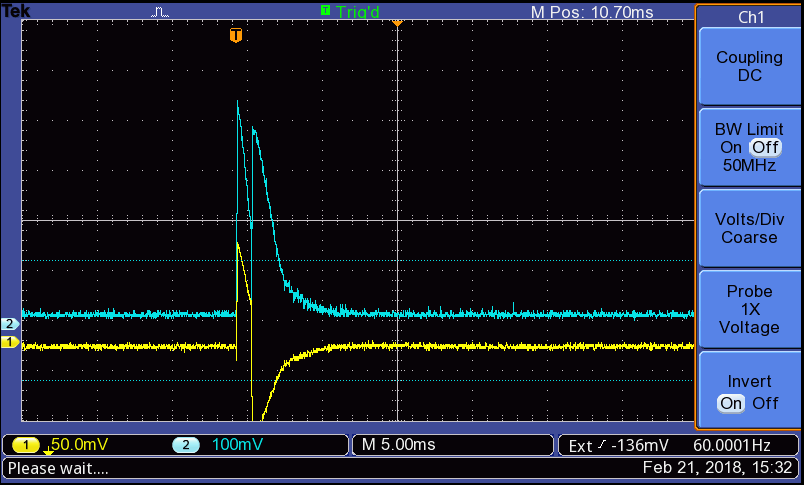
\includegraphics[scale=0.8]{Bilder/F0003TEK.PNG}
\caption{Ergebnis einer einzelnen Messung zur Bestimmung von T1. Die blaue Kurve zeigt das zu untersuchende Signal.}
\label{fig:MessungT1_Beispiel}
\end{figure}

Für die Messung von $T_1$ werden die Spins mit einem $\pi$-Puls umgedreht. Nach einer Wartezeit $\tau$, werden die restlichen, noch in der umgedrehten Position befindlichen Spins mit einem $\pi /2$-Puls in die x-y-Ebene gedreht, um dort vermessen zu werden. Das Ergebnis einer solchen Messung ist beispielhaft in Abbildung \ref{fig:MessungT1_Beispiel} gezeigt (das blau dargestellte Signal wird betrachtet). Der erste Peak ist der Rest des $\pi$-Pulses. Der zweite Peak ist der Free Induction Decay (FID) nach dem $\pi /2$-Puls. \\
Für die Bestimmung von $T_1$ wird die Wartezeit zwischen den beiden Pulse durchgefahren und die relative Höhe des FID zur Höhe des $\pi$-Pulses bestimmt. Die Erwartung ist ein exponentieller Abfall:
\begin{equation}
\label{eq:T1_Exponentialfunktion}
U_{rel} (t) := \dfrac{U_{FID} (t)}{U_0} = 1 - 2 e^{-\frac{t}{T_1}}
\end{equation}
Es wurden die Einstellungen verwendet, die sich bei der Optimierung der Einstellungen ergeben haben.

\subsection{Messung von $T_2$}

Für die Messung von $T_2$ werden die Spins mit einem  $\dfrac{\pi}{2}$ Puls in die x-y-Ebene gedreht. Durch Inhomogenitäten im Magnetfeld präzedieren die Spins allerdings unterschiedlich schnell, wodurch der Magnetisierungsvektor verschmiert. Deswegen wird nach einer Wartezeit $\tau$ ein $\pi$ Puls angelegt, der die Spins innerhalb der Ebene spiegelt und somit die Verschmierungsrichtung umdreht. Dadurch entsteht nach einer Zeit von insgesamt $2 \tau$ ein Spinecho. \\ 
\\
Um außerdem möglichen Diffusionsprozessen entgegen zu wirken gibt es nun 2 unterschiedliche Verfahren:

\subparagraph{Carr-Purcell-Pulssequenz}
Bei diesem Verfahren wird nach den anfänglichen $\dfrac{\pi}{2}$ und $\pi$ Pulsen alle  $2 \tau$ ein neuer $\pi$ Puls angelegt. Dadurch erhält man mehrere Spinechos bei einer Pulssequenz. Durch die wesentlich schnellere Durchführung werden so Diffusionseffekte minimiert.
\subparagraph{Meiboom-Gill-Pulssequenz}
Dieses Verfahren besteht aus exakt derselben Pulssequenz, wie das Carr-Purcell-Verfahren. Der große Unterschied ist aber, dass  die $\pi$ Pulse um $90^{\circ}$ zum anfänglichen $\dfrac{\pi}{2}$ Puls verschoben ist. Wurde der $\pi$ Puls beim C-P-Verfahren also in x-Richtung (im ruhendem System) angelegt, so befindet er sich jetzt in y-Richtung.\\
Dies sorgt dafür, dass sich Verchiebungen von der x-y Ebene beim $\pi$ Puls nicht immer weiter aufaddieren.
\\
Es wurden zu beiden Methoden Datensätze für verschiedene $\tau$ aufgezeichnet, um bei der Auswertung entscheiden zu können, welche Methode die besseren Ergebnisse liefert.\\
Dabei wird das $\tau$ möglichst klein gewählt, allerdings groß genug, damit die Peaks nicht untereinander Interferieren und noch gut erkennbar sind. Im vorliegendem Aufbau ergab ein $\tau$ zwischen 4-7ms ein gutes Bild.\\

\begin{figure}
\centering
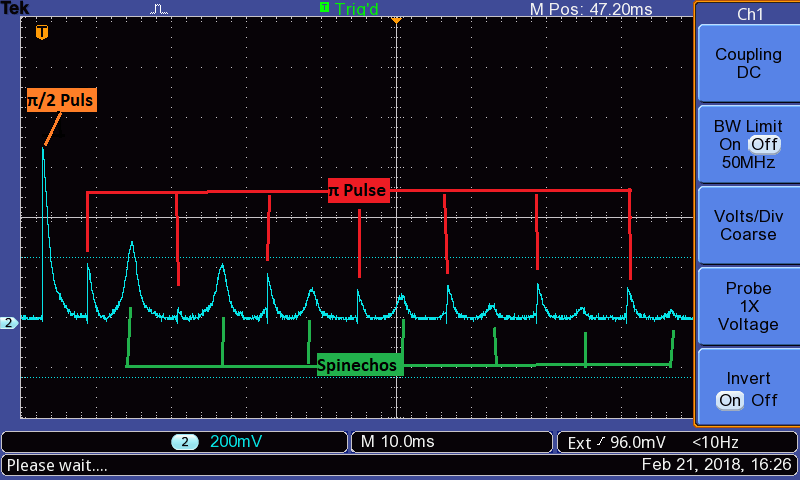
\includegraphics[scale=0.8]{Bilder/T2Beispiel.png}
\caption{Datensatz zur Bestimmung von $T_2$ beispielhaft für die Meiboom-Gill-Sequenz mit $\tau = 6ms$. Es wurde gekennzeichnet, um welche Art von Peak es sich handelt. }
\label{fig:T2Beispiel}
\end{figure}


\section{Ergebnisse}

\subsection{Vorversuche}

\subsubsection{Leiterschleife}

Für den Vorversuch musste die Leiterschleife vermessen werden. Die verwendete Leiterschleife besteht aus $N=2$ Windungen und hat eine Querschnittsfläche von 
\begin{equation*}
A =  \SI{0.35\pm 0.01}{cm} \cdot \SI{0.42\pm 0.01}{cm} = \SI{0.147\pm 0.005}{cm^2}.
\end{equation*}
Bei eriner eingestellten Frequenz von $f = \SI{21.571}{Mhz}$ wurde die gemessene Spannugnsamplitude maximal. Die maximale Spannung wurde bei $U =\SI{23.6\pm 0.2}{V}$ abgelesen. Daraus ergibt sich mithilfe von Formel \ref{B1} ein Wechselmagnetfeld von 
\begin{equation*}
\boxed{B_1 = \SI{2.96\pm 0.10}{mT}}
\end{equation*}
und daraus eine ungefähre $\pi /2$-Pulsdauer von
\begin{equation*}
\boxed{T_{\pi /2} = \SI{1.98\pm 0.07}{\mu s}}
\end{equation*}
\subsubsection{Optimierung der Einstellungen}
Bei der Feineinstellung wurde eine optimale Frequenz von  $f = \SI{21.590}{Mhz}$ gefunden. Die Dauer des $\pi / 2 $-Pulses musste ebenfalls auf $\SI{2.56}{\mu s}$, bzw. auf $\SI{5.13}{\mu s}$ für den $\pi$-Puls korrigiert werden, um einen möglichst großen Peak zu sehen. Die Abweichung vom errechneten Wert für die Pulslänge kann daran liegen, dass die Glaswand des Probenbehälters, bzw. die Probe selbst das Magnetfeld abschwächt.\\
Die Änderungen der Lamorfrequenz durch Temperaturschwankungen etc. fanden auf der 4.Nachkommastelle statt. Sie beeinflussen den Versuch also nicht nennenswert.

\subsection{$T_1$}
Bei den Messungen zu $T_1$ wird immer nur der Betrag des FID-Signals gemessen, daher muss der Teil der Messwerte, die vor dem Nulldurchgang liegen noch mit dem Faktor (-1) multipliziert werden. In Tabelle \ref{tab:T1_Daten} ist dies bereits geschehen. Genauso ist der Offset bereits korrigiert. Die Fehler auf die Puls- und FID-Höhe werden in dem Abschnitt zur Rauschmessung erklärt. Der Fehler auf die Zeit entspricht dem Ablesefehler des Maximums. Dieser entspricht 8 Digitalisierungsschritten, wobei eine Gleichverteilung angenommen wird:
\begin{equation*}
\sigma _{\tau} = \dfrac{8 \cdot \Delta}{\sqrt{12}} = \dfrac{8 \cdot \frac{45 ms}{2500}}{\sqrt{12}} \approx 0.042 ms
\end{equation*}
Ab einem gewissen Punkt musste die Auflösung der Zeitachse des Oszilloskops verringert werden, damit der FID weiterhin sichtbar bleibt. Daher wird der Fehler auf $\tau$ dann um Faktor 5 größer.

\begin{table}
\centering
\begin{tabular}{|c|c|c|}
\hline 
Pulshöhe [mV] & FID-Höhe [mV] & $\tau$ [ms] \\ 
\hline 
428 $\pm$ 4 & -376 $\pm$ 4 & 0.918 $\pm$ 0.042 \\ 
\hline 
432 $\pm$ 4 & -360 $\pm$ 4 & 1.800 $\pm$ 0.042 \\ 
\hline 
432 $\pm$ 4 & -336 $\pm$ 4 & 2.700 $\pm$ 0.042 \\ 
\hline 
452 $\pm$ 4 & -308 $\pm$ 4 & 3.618 $\pm$ 0.042 \\ 
\hline 
452 $\pm$ 4 & -276 $\pm$ 4 & 4.554 $\pm$ 0.042 \\ 
\hline 
432 $\pm$ 4 & -248 $\pm$ 4 & 5.436 $\pm$ 0.042 \\ 
\hline 
440 $\pm$ 4 & -216 $\pm$ 4 & 6.300 $\pm$ 0.042 \\ 
\hline 
428 $\pm$ 4 & -184 $\pm$ 4 & 7.290 $\pm$ 0.042 \\ 
\hline 
440 $\pm$ 4 & -156 $\pm$ 4 & 8.154 $\pm$ 0.042 \\ 
\hline 
436 $\pm$ 4 & -116 $\pm$ 4 & 9.036 $\pm$ 0.042 \\ 
\hline 
436 $\pm$ 4 & -104 $\pm$ 4 & 9.954 $\pm$ 0.042 \\ 
\hline 
432 $\pm$ 4 & -72 $\pm$ 4 & 10.854 $\pm$ 0.042 \\ 
\hline 
424 $\pm$ 4 & -52 $\pm$ 4 & 11.862 $\pm$ 0.042 \\ 
\hline 
436 $\pm$ 4 & -32 $\pm$ 4 & 12.978 $\pm$ 0.042 \\ 
\hline 
428 $\pm$ 4 & -20 $\pm$ 4 & 13.428 $\pm$ 0.042 \\ 
\hline 
420 $\pm$ 4 & -16 $\pm$ 4 & 14.040 $\pm$ 0.042 \\ 
\hline 
424 $\pm$ 4 & -12 $\pm$ 4 & 14.148 $\pm$ 0.042 \\ 
\hline 
432 $\pm$ 4 & -8 $\pm$ 4 & 14.490 $\pm$ 0.042 \\ 
\hline 
428 $\pm$ 4 & 8 $\pm$ 4 & 14.850 $\pm$ 0.042 \\ 
\hline 
428 $\pm$ 4 & 24 $\pm$ 4 & 15.300 $\pm$ 0.042 \\ 
\hline 
420 $\pm$ 4 & 20 $\pm$ 4 & 15.516 $\pm$ 0.042 \\ 
\hline 
420 $\pm$ 4 & 32 $\pm$ 4 & 15.858 $\pm$ 0.042 \\ 
\hline 
428 $\pm$ 4 & 40 $\pm$ 4 & 16.326 $\pm$ 0.042 \\ 
\hline 
420 $\pm$ 4 & 36 $\pm$ 4 & 17.118 $\pm$ 0.042 \\ 
\hline 
428 $\pm$ 4 & 60 $\pm$ 4 & 18.000 $\pm$ 0.042 \\ 
\hline 
424 $\pm$ 4 & 88 $\pm$ 4 & 18.864 $\pm$ 0.042 \\ 
\hline 
424 $\pm$ 4 & 108 $\pm$ 4 & 19.818 $\pm$ 0.042 \\ 
\hline 
432 $\pm$ 4 & 116 $\pm$ 4 & 20.718 $\pm$ 0.042 \\ 
\hline 
424 $\pm$ 4 & 140 $\pm$ 4 & 21.636 $\pm$ 0.042 \\ 
\hline 
432 $\pm$ 4 & 156 $\pm$ 4 & 22.500 $\pm$ 0.042 \\ 
\hline 
420 $\pm$ 4 & 176 $\pm$ 4 & 23.400 $\pm$ 0.042 \\ 
\hline 
412 $\pm$ 4 & 180 $\pm$ 4 & 24.336 $\pm$ 0.042 \\ 
\hline 
424 $\pm$ 4 & 192 $\pm$ 4 & 25.218 $\pm$ 0.042 \\ 
\hline 
416 $\pm$ 4 & 208 $\pm$ 4 & 26.100 $\pm$ 0.042 \\ 
\hline 
424 $\pm$ 4 & 228 $\pm$ 4 & 27.090 $\pm$ 0.042 \\ 
\hline 
396 $\pm$ 4 & 232 $\pm$ 4 & 27.990 $\pm$ 0.042 \\ 
\hline 
400 $\pm$ 4 & 240 $\pm$ 4 & 28.800 $\pm$ 0.042 \\ 
\hline 
404 $\pm$ 4 & 252 $\pm$ 4 & 29.700 $\pm$ 0.208 \\ 
\hline 
412 $\pm$ 4 & 276 $\pm$ 4 & 30.600 $\pm$ 0.208 \\ 
\hline 
384 $\pm$ 4 & 280 $\pm$ 4 & 30.690 $\pm$ 0.208 \\ 
\hline 
396 $\pm$ 4 & 272 $\pm$ 4 & 31.500 $\pm$ 0.208 \\ 
\hline 
\end{tabular} 
\caption{Messwerte der Höhen des $\pi /2$-Pulses und des FID s beim Durchfahren von $\tau$ zur Bestimmung von $T_1$.}
\label{tab:T1_Daten}
\end{table}


\subsubsection{Rauschmessung}
Wie in Abbildung \ref{fig:MessungT1_Beispiel} gut zu erkennen ist, ist ein deutliches Hintergrundrauschen vorhanden. Aus diesem lässt sich ein Offset bestimmen, der zur Korrektur der Höhen wichtig ist, und ein statistischer Fehler auf die Spannungsmessung. Die Ergebnisse sind:
\begin{equation*}
\sigma _{Rauschmessung} = 4 mV
\end{equation*}
\begin{equation*}
U_{offset} = 20 mV
\end{equation*}
Zusätzlich zum Fehler aus der Rauschmessung muss noch der Ablesefehler berücksichtigt werden. Diesen erhält man aus der Digitalisierung unter Annahme einer Gleichverteilung:
\begin{equation*}
\sigma _{Digitalisierung} = \dfrac{\Delta}{\sqrt{12}} = \dfrac{4 mV}{\sqrt{12}}
\end{equation*}
Damit ergibt sich der Fehler auf die Spannungsmessung zu:
\begin{equation*}
\sigma _U = \sqrt{\left(\sigma _{Rauschmessung} \right)^2 + \left(\sigma _{Digitalisierung} \right)^2}
\end{equation*}
Dieser Fehler kann nun mittels Gl. \ref{eq:T1_Exponentialfunktion} auf die relative Höhe fortgepflanzt werden:
\begin{equation*}
\sigma _{U_{rel}} = \sigma _U \cdot \sqrt{\left(\dfrac{1}{U_{Puls} - U_{offset}}\right)^2 + \left(\dfrac{U_{FID} - U_{offset}}{(U_{Puls} - U_{offset})^2}\right)^2}
\end{equation*}


\subsubsection{Zero-crossing-point-Methode}

\begin{figure}
\centering
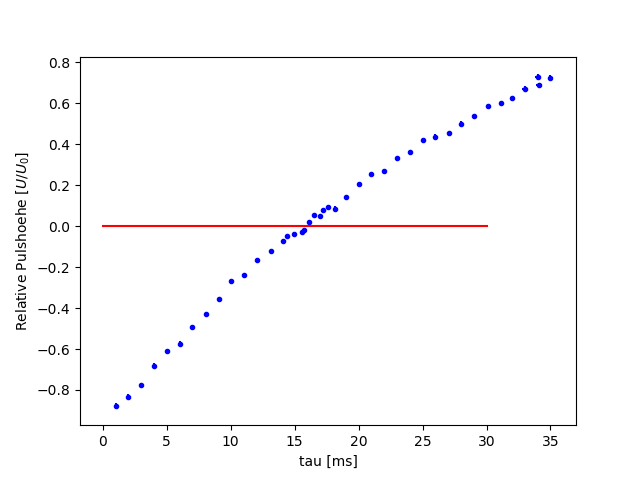
\includegraphics[scale=0.7]{Bilder/T1_ZeroCrossingPoint.PNG}
\caption{Veranschaulichung des sogenannten zero-crossing-points.}
\label{fig:T1_Zero_Crossing}
\end{figure}

Anhand von Gl. \ref{eq:T1_Exponentialfunktion} lässt sich leicht ersehen, dass aus dem Punkt an dem die Daten die Nulllinie durchqueren $T_1$ abgeschätzt werden kann als:
\begin{equation*}
T_1 = \dfrac{1}{ln(2)} \cdot T_{U_{rel} = 0}
\end{equation*}
Abbildung \ref{fig:T1_Zero_Crossing} veranschaulicht den zero-crossing-point. Dabei zeigt sie gleichzeitig auch die große Unsicherheit: Um den zero-crossing-point gibt es viele Punkte, die sehr nah an der Null sind. \\ 
Anhand der Daten ist gut ersichtlich, dass der Nulldurchgang irgendwo zwischen den Werten $T_{U_{rel} < 0} = 13.428ms$ und $T_{U_{rel} > 0} = 15.516ms$ liegt. Damit ergibt sich der Messwert für $T_1$ zu:
\begin{equation*}
T_1 = \dfrac{1}{ln(2)} \cdot \dfrac{T_{U_{rel} > 0} + T_{U_{rel} < 0}}{2} = 20.879 ms
\end{equation*}
\begin{equation*}
\sigma _{T_1} = \dfrac{1}{ln(2)} \cdot \dfrac{T_{U_{rel} > 0} - T_{U_{rel} < 0}}{\sqrt{12}} = 0.870 ms
\end{equation*}

\subsubsection{Linearer Fit an halblogarithmischer Auftragung}

\begin{figure}
\centering
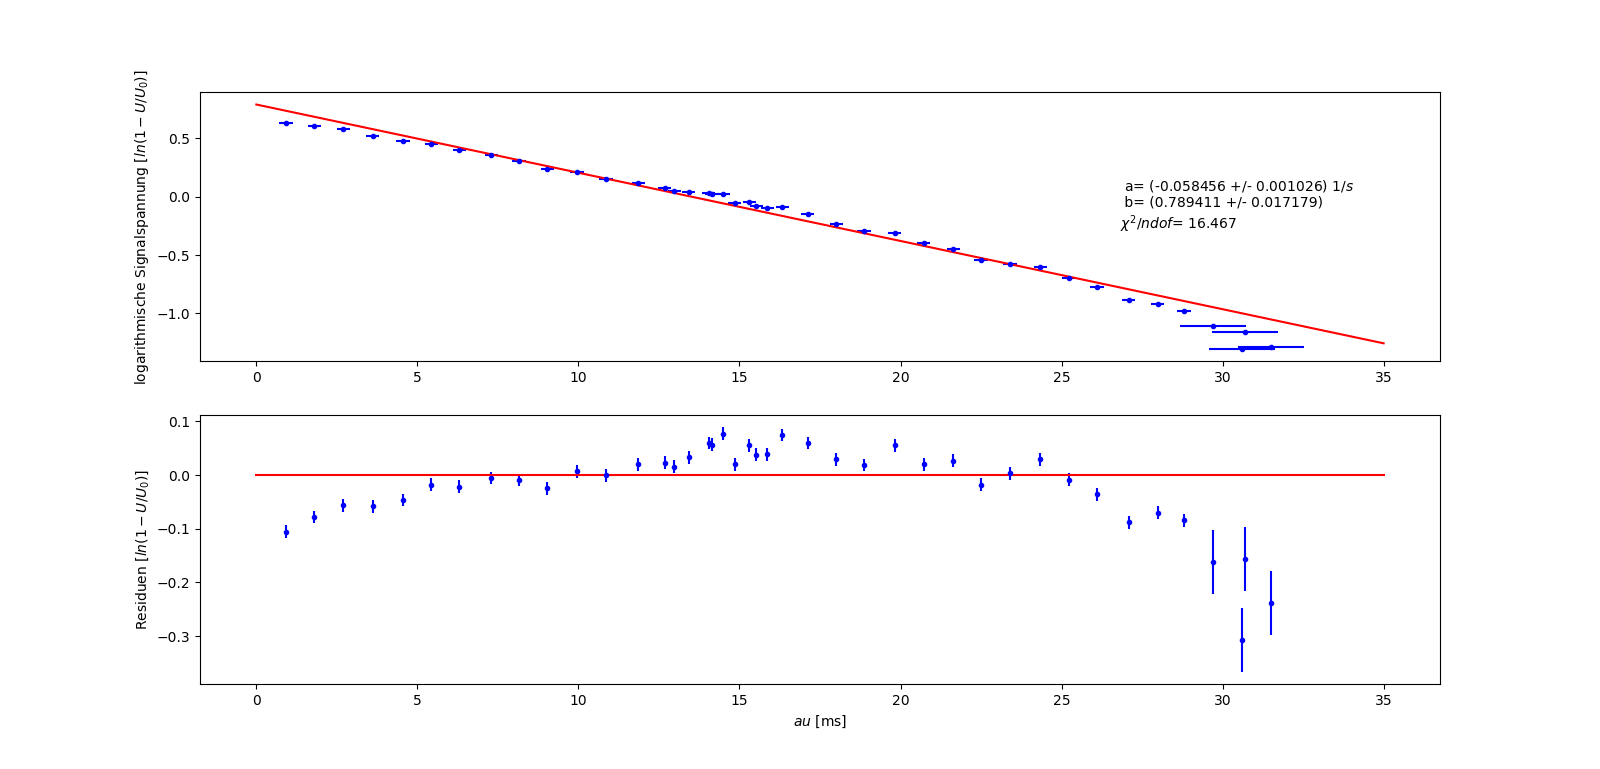
\includegraphics[scale=0.7]{Bilder/T1_linFit_halblog.PNG}
\caption{Lineare Regression an Auftragung von $ln\left(\dfrac{1-U_{rel}}{2}\right)$ gegen die Zeit t.}
\label{fig:T1_linFit}
\end{figure}

Formt man Gl. \ref{eq:T1_Exponentialfunktion} zu einer linearen Funktion um, ergibt sich:
\begin{equation}
ln\left(\dfrac{1 - U_{rel} (t)}{2}\right) = -\dfrac{t}{T_1}
\label{eq:T1_linFunktion}
\end{equation}
Daher kann durch geeignete Auftragung eine lineare Funktion an die Daten gefittet werden. Mittels Fehlerfortpflanzung ergibt sich für die Fehler auf die Y-Koordinate:
\begin{equation}
\sigma _y = \sigma _{U_{rel}} \cdot \dfrac{1}{1 - U_{rel}}
\end{equation}
Der Fehler auf die X-Koordinate entspricht dabei einfach dem Fehler auf die Zeitmessung.\\
Abbildung \ref{fig:T1_linFit} zeigt den linearen Fit an der halblogarithmischen Auftragung. Daraus ergibt sich für $T_1$ und den Fehler darauf:
\begin{equation*}
T_1 = -\dfrac{1}{a} = 19.661 ms
\end{equation*}
\begin{equation*}
\sigma _{T_1} = T_1 \cdot \dfrac{-\sigma _a}{a} = 0.216 ms
\end{equation*}

\subsubsection{Exponentialfit}

\begin{figure}
\centering
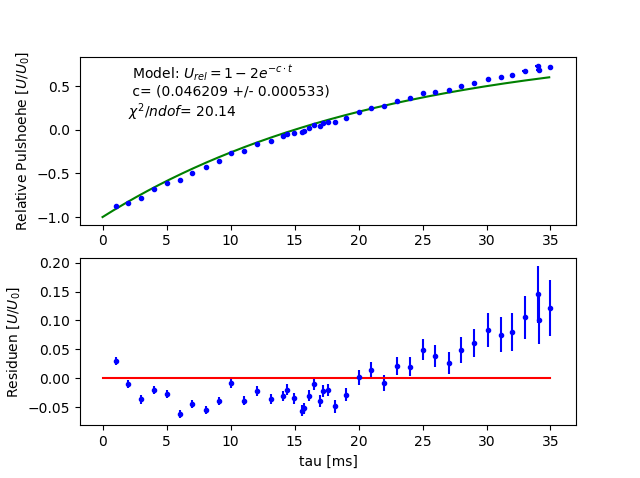
\includegraphics[scale=0.7]{Bilder/T1_expFit.PNG}
\caption{Fit einer Exponentialfunktion an die Daten.}
\label{fig:T1_expFit}
\end{figure}

Alternativ zum linearen Fit bei geeigneter Auftragung kann auch an die Rohdaten direkt eine Exponentialfunktion  wie in Gl. \ref{eq:T1_Exponentialfunktion} angepasst werden. Dazu wird das Ergebnis aus dem linearen Fit als Startwert verwendet. Abbildung \ref{fig:T1_expFit} zeigt den Fit. Daraus bestimmt sich $T_1$ und der Fehler darauf zu:
\begin{equation*}
T_1 = \dfrac{1}{c} = 19.477 ms
\end{equation*}
\begin{equation*}
\sigma _{T_1} = T_1 \cdot \dfrac{\sigma _c}{c} = 0.215 ms
\end{equation*}

\subsubsection{Systematische Fehler} 
Da die Drehung der Spins um das effektive Magnetfeld geschieht und die Messung der Magnetisierung in einer bestimmten Ebene stattfindet, ist es für die Messung wichtig, dass das effektive Magnetfeld richtig ausgerichtet ist und dass die Pulslänge richtig eingestellt ist. Die hohe Temperaturabhängigkeit des Aufbaus hat zur Folge, dass Temperaturschwankungen für ein im Vergleich zur idealen Ausrichtung verändertes effektives Magnetfeld und damit eine veränderte Frequenz und eine veränderte Pulslänge führen. Daher hat die Temperatur einen sehr großen Einfluss auf die Messung des Betrags der Magnetisierung. \\
Einen ähnlichen Effekt erhält man durch Spins, die vor der Pulssequenz nicht exakt in z-Richtung ausgerichtet sind. Diese Spins werden auch bei der richtigen Frequenz und der richtigen Pulslänge nicht exakt in die x-y-Ebene gedreht, sodass sie einen kleineren Teil zur gemessenen Magnetisierung beitragen. \\
Hinzu kommen lokale Inhomogenitäten der Magnetfelder, die ebenfalls dafür sorgen, dass einzelne Spins nicht in die x-y-Ebene gedreht werden und damit nur einen kleineren Teil zur gemessenen Magnetisierung beitragen.

\subsubsection{Zusammenfassung}

\begin{table}
\centering
\begin{tabular}{|c|c|c|c|}
\hline 
Methode & $T_1$ [mV] & $\sigma _{T_1}$ [ms] & $\chi ^2$ /ndof \\ 
\hline 
Zero-crossing-point & 20.879 & 0.870 & - \\ 
\hline 
Linearer Fit & 19.661 & 0.216 & 4.489 \\ 
\hline 
Exponentialfit & 19.477 & 0.215 & 20.140 \\ 
\hline 
\end{tabular} 
\caption{Ergebnisse für $T_1$ aus den unterschiedlichen Auswertungsmethoden angewandt auf dieselben Daten.}
\label{tab:T1_Ergebnisse}
\end{table}

Tabelle \ref{tab:T1_Ergebnisse} zeigt nochmal zusammengefasst die Ergebnisse aus den Auswertungsmethoden. Dabei ist deutlich erkennbar, dass die Ergebnisse zwar nahe beieinander liegen, jedoch nur die beiden Ergebnisse aus den Anpassungen innerhalb ihrer Fehler übereinstimmen. Da alle Auswertungsmethoden dieselbe Messreihe verwenden, sind die systematischen Fehler identisch.\\
Da die Messung immer nur den Betrag ergibt und deswegen der Nulldurchgang nachträglich eingefügt werden muss, liefert die zero-crossing-point Methode nur eine Abschätzung für den Wert von $T_1$. Die beiden Anpassungen sind genauer, da hier der Nulldurchgang nur eine untergeordnete Rolle spielt. Anhand der Darstellungen ist deutlich erkennbar, dass die Anpassungen in einem Teilbereich gut funktionieren und ab einem gewissen Punkt die Daten deutlich abweichen. Dabei ist anhand des $\chi ^2 /ndof$ leicht erkennbar, dass der lineare Fit besser funktioniert hat als Exponentialfit.


\subsection{T2}
\subsubsection{Messdaten}\label{sec:T2messdaten}
\begin{figure}
\centering
\includegraphics[scale=0.8]{Bilder/T2CP.png}
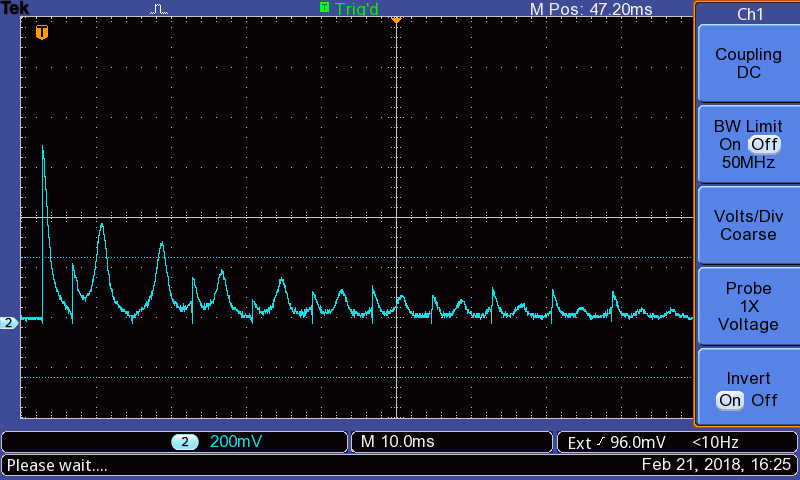
\includegraphics[scale=0.8]{Bilder/T2MG.png}
\caption{Ergebnisse der Pulssequenzen zur Bestimmung von $T_2$ mit $\tau = 4ms$ und verstelltem Pulslängen. \textbf{Oben}: Carr-Purcell-Verfahren. \textbf{Unten}: Meiboom-Gill-Verfahren. Auffällig sind die sichtbaren $\pi$ Pulse und das Fehlen des 3.Spinechos beim C-P-Verfahren.}
\label{fig:T2Daten}
\end{figure}

Die ersten Messungen für $T_2$ sind in Abbildung \ref{fig:T2Daten} für beide Verfahren beispielhaft dargestellt.\\
Bei dieser Messreihe ist auffällig, dass die $\pi$ Pulse und deren FID sichtbar sind, was bei idealen Einstellungen und Spinverhalten nicht der Fall sein sollte. Außeredem verschwindet bei der C-P-Methode das 3.Spinecho.
\paragraph{mögliche systematische Fehler:}

Das Auftreten der $\pi$ Pulse kann verschiedene Ursachen haben. Einerseits kann die RF-Kreisfrequenz falsch eingestellt sein. Dadurch befindet sich das Magnetfeld bei den Pulsen nicht in der x-y Ebene, wodurch die Spinausrichtung nach einem $\pi$ Puls eine horizontale Komponente hat, welche natürlich gemessen weir.\\
Es kann außerdem sein, dass die Pulslängen falsch eingestellt waren. Durch eine Kombination mit der falschen Frequenz kann dies dazu führen, dass der $\pi$ Puls die in der Durchführung beschriebene Verschmierung teilweise aufhebt, wodurch ein messbarer Peak entsteht.\\
Falsch eingestellte Pulslängen würden auch das Fehlen des 3.Spinechos  bei der C-P-Methode erklären, da sich die Abweichungen von der x-y Ebene hier wie oben beschrieben aufaddieren und der Spinvektor somit nach mehreren $\pi$ Pulsen im Extremfall in z-Richtung zeigt und somit nicht gemessen werden kann.\\
\\
Um diese Effekte zu minimieren wurde eine zweite Messreihe aufgenommen, bei der die Frequenz nochmals neu kalibriert wurde und die Pulslängen so angepasst wurden, dass die $\pi$ Pulse möglichst klein ausfallen. Diese Messreihe ist beispielhaft in Abbildung \ref{fig:T2Datenalt} zu sehen.\\
Es ist dort wie erwartet zu sehen, dass die Peaks bei der C-P-Methode wegen der Abweichung von der x-y Ebene schneller abfallen. Dies ist ein unerwünschter Effekt, der das Ergebnis unter Umständen stark beeinflusst. Außerdem sind die Peaks ab einer gewissen Ordnung sehr klein und sogar teilweise gar nicht mehr sichtbar, was das Ergebnis deutlich ungenauer machen würde.\\
Deswegen wurde entschieden die Daten des Meiboom-Gill-Verfahrens für die Auswertung zu benutzen.
\begin{figure}
\centering
\includegraphics[scale=0.8]{Bilder/T2CPalt.png}
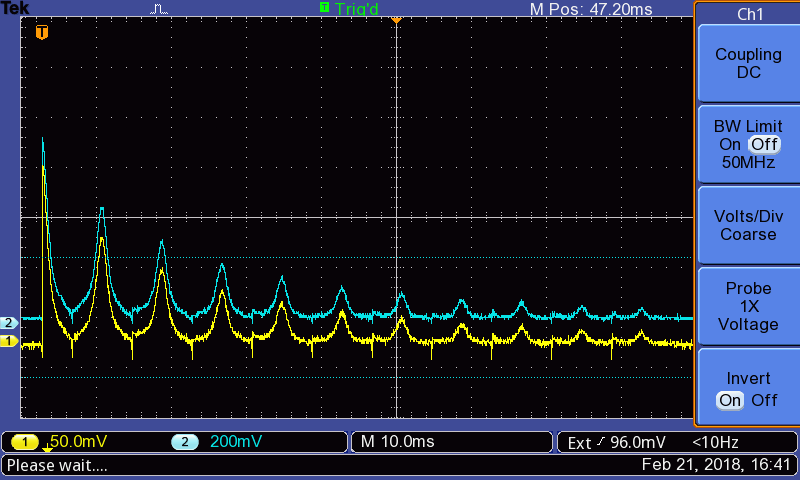
\includegraphics[scale=0.8]{Bilder/T2MGalt.png}
\caption{Ergebnisse für $T_2$ mit angepasster Frequenz und Pulslänge für $\tau = 4ms$. \textbf{Oben}: Carr-Purcell-Verfahren. \textbf{Unten}: Meiboom-Gill-Verfahren. Für die Auswertung relevant ist nur die "blaue" Kurve von Channel 2, welche die Amplitude des Messsignals beschreibt.}
\label{fig:T2Datenalt}
\end{figure}

\subsubsection{Peakbestimmung}
Mithilfe eines Programmes wurden die vom Oszilloskop gegebenen Datensätze eingelesen.
Es wurde wie bei der Bestimmung von $T_1$ wieder eine Rauschmessung durchgeführt.
Diese ergab einen Offset von $U_{Offset} = 20.6mV$ und eine Schwankung von $\sigma = 4mV$.\\
Die Peakhöhe und Lage wurde durch eine lokale Maximumsbestimmung in der Nähe der Peaks durchgeführt.\\
Dabei wurde der Peak des $\pi/2$ Pulses ausgenommen, da dieser nicht durch ein Spinecho entsteht und der Puls somit das Ergebnis verfälschen könnte.\\
Bei allen Datensätzen wurde eine Zeitskala von 10ms und eine Höhenskala von 200mV gewählt. Bei diesen Skalen betragen die Digitalisierungsfehler 8mV und 0.04ms.\\
Da das Maximum oft über mehrere Digitalisierungsschritte verteilt war, wurde angenommen, dass das wahre Maximum gleichverteilt zwischen diesen Schritten liegt. Eine gute Wahl der Maximumsbreite betrug $\Delta t = 0.16ms$.\\
Damit ergibt sich eine Ableseungenauigkeit auf die Lage von

\begin{equation*}
\sigma_t = \dfrac{\Delta t}{\sqrt{12}} \approx 0.05ms
\end{equation*}

Der Fehler auf die Peakhöhe ergibt sich durch die Schwankung der Werte innerhalb der Maximumsbreite. In diesem Fehler steckt sowohl der Digitalisierungsfehler, als auch der Fehler durch das Rauschen, weswegen diese Fehler nicht mehr extra einbezogen werden müssen.

\begin{table}
\centering
\begin{tabular}{|c|c|}
\hline 
Position[ms] & Höhe[mV]\\ 
\hline
$ 8.17 \pm 0.05 $ & $ 437.01 \pm 11.31 $ \\
\hline
$ 16.08 \pm 0.05 $ & $ 309.01 \pm 6.53 $ \\
\hline
$ 24.06 \pm 0.05 $ & $ 213.01 \pm 6.53 $ \\
\hline
$ 32.04 \pm 0.05 $ & $ 167.01 \pm 3.77 $ \\
\hline
$ 40.03 \pm 0.05 $ & $ 123.01 \pm 7.54 $ \\
\hline
$ 48.03 \pm 0.05 $ & $ 103.01 \pm 3.77 $ \\
\hline
$ 56.02 \pm 0.05 $ & $ 71.01 \pm 3.77 $ \\
\hline
$ 64.02 \pm 0.05 $ & $ 67.01 \pm 7.54 $ \\
\hline
$ 72.02 \pm 0.05 $ & $ 47.01 \pm 3.77 $ \\
\hline
$ 80.02 \pm 0.05 $ & $ 39.01 \pm 3.77 $ \\
\hline
\end{tabular}
\caption{Gefundene Peaks für $\tau = 4ms$ }
\end{table}

\subsubsection{Exponentialfit}

\begin{figure}
\centering
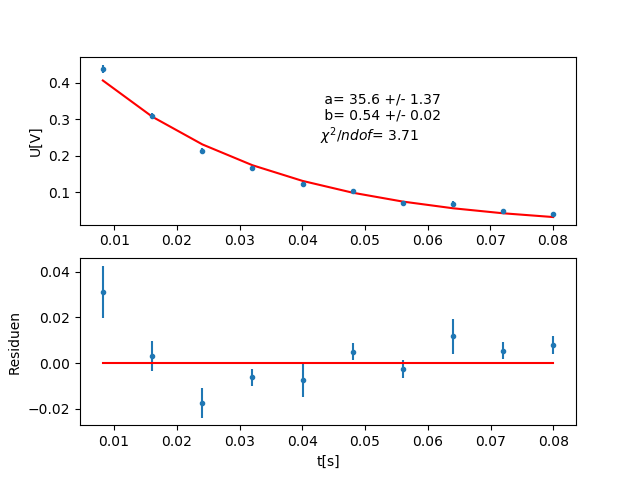
\includegraphics[scale=0.9]{Bilder/T2exp.png}
\caption{Exponentialfit}
\label{fig:T2exp}
\end{figure}

An die gefundenen Peaks wird nun eine Exponentialfunktion der Form

\begin{equation}
y = b \cdot e^{-a\cdot t}
\end{equation}
gefittet. Dies ist in Abbildung \ref{fig:T2exp} dargestellt.\\
Aus den gefundenen Werten berechnet sich $T_2$ durch 
\begin{equation*}
T_2 = \dfrac{1}{a} = 28.1ms
\end{equation*}
und der Fehler durch
\begin{equation*}
\sigma_{T_2} = \dfrac{1}{a^2} \cdot \sigma_a = 1.1ms
\end{equation*}

\subsubsection{Linearer Fit an Halblogarythmischer Auftragung}

\begin{figure}
\centering
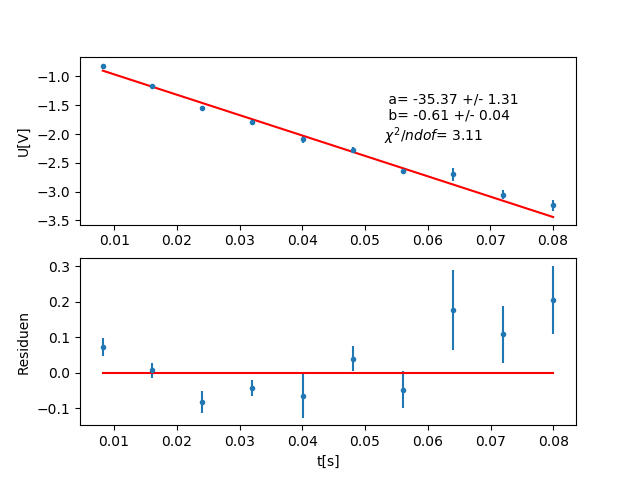
\includegraphics[scale=0.9]{Bilder/T2lin.png}
\caption{Linearer Fit}
\label{fig:T2lin}
\end{figure}

Nun werden die Spannungswerte logarithmisiert und eine lineare Funktion an die Daten gefittet:
\begin{equation}
y = a \cdot t + b
\end{equation}
Daraus erhält man $T_2$ wieder durch 
\begin{equation*}
T_2 = \dfrac{-1}{a} = 28.3ms
\end{equation*}
und den Fehler durch
\begin{equation*}
\sigma_{T_2} = \dfrac{1}{a^2} \cdot \sigma_a = 1.0ms
\end{equation*}

\subsubsection{Auswertung weiterer Messreihen und Zusammenfassung}

Um mögliche Systematiken abschätzen zu können wurden mit den oben beschriebenen Methoden weitere Datensätze ausgewertet. Alle Ergebnisse sind in Tabelle \ref{T2zusammenfassung} aufgelistet. Die dazugehörigen Anpassungen befinden sich im Anhang.
Zuerst wurde die Messung mit dem Meiboom-Gill Verfahren für verschiedene $\tau$ wiederholt, um ein genaueres Resultat zu bekommen und mögliche statistische Schwankungen und Fehlmessungen zwischen verschiedenen Messungen zu eliminieren.\\
Die Ergebnisse stimmen sowohl für verschiedene Messreihen als auch für die beiden verschiedenen Auswertungsmethoden innerhalb ihrer Fehler überein. 	Eine gewichtete Mittelung über die vier Messungen liefert unser Endergebnis:

\begin{equation*}
\boxed{T_{2, Exponential} = (27.6\pm 0.5)ms}
\end{equation*}
\begin{equation*}
\boxed{T_{2, Linear} = (27.8\pm 0.5)ms}
\end{equation*}\\

Anhand der Messreihe, bei der Frequenz und Pulslängen verstellt waren, kann außerdem der Einfluss von verstellten Parametern beobachtet werden. Es ist auffällig, dass die Ergebnisse der einzelnen Messungen sehr viel stärker schwanken und im Mittel mit $T_2 = (28.9\pm0.8)ms$ größer sind. Dies war zu erwarten, da sich die Magnetisierung hier durch die in Kapitel \ref{sec:T2messdaten} beschriebenen Effekte unkontrollierter verhält.\\
\\
Zuletzt wurde noch das Carr-Purcell-Verfahren ausgewertet. Es ist zu sehen, dass dieses Verfahren eine wesentlich kleineres $\tau$ liefert, da die Pulslängen nicht genau genug eingestellt werden konnten. Bei stark verstellten Parametern kann man die Daten sogar nicht mehr wirklich auswerten, was an dem deutlich größeren $\chi^2/ndof$ der alternativen C-P-Messung (vgl. Tabelle \ref{T2zusammenfassung}) zu sehen ist.

\begin{table}
\begin{tabular}{|c|c|c||c|c||c|c|}
\hline
Verfahren & $\tau [ms]$ & Peaks &  $T_2$ (Exponentialfit) & $\chi^2/ndof$ &$T_2$ (Linerarer Fit) & $\chi^2/ndof$\\
\hline
M-G & $4$ & 10 & $ 28.1 \pm 1.1 $ & $ 3.71 $ & $ 28.3 \pm 1.0 $ & $ 3.11 $ \\
\hline
M-G & $5$ & 9 & $ 27.4 \pm 1.0 $ & $ 2.73 $ & $ 27.7 \pm 1.0 $ & $ 2.48 $ \\
\hline
M-G & $6$ & 7 & $ 27.3 \pm 0.8 $ & $ 1.83 $ & $ 27.5 \pm 0.8 $ & $ 1.43 $ \\
\hline
M-G & $7$ & 6 & $ 27.7 \pm 1.3 $ & $ 2.53 $ & $ 27.9 \pm 1.3 $ & $ 1.83 $ \\
\hline
\hline
M-G(alt.) & $4$ & 10 & $ 27.3 \pm 1.0 $ & $ 2.4 $ & $ 27.4 \pm 0.9 $ & $ 1.89 $ \\
\hline
M-G(alt.) & $5$ & 9 & $ 30.7 \pm 1.1 $ & $ 2.49 $ & $ 31.0 \pm 1.1 $ & $ 1.8 $ \\
\hline
M-G(alt.) & $6$ & 7 & $ 28.6 \pm 1.3 $ & $ 1.71 $ & $ 28.8 \pm 1.2 $ & $ 1.15 $ \\
\hline
M-G(alt.) & $7$ & 6 & $ 29.5 \pm 1.9 $ & $ 4.95 $ & $ 29.8 \pm 2.0 $ & $ 3.22 $ \\
\hline
\hline
C-P & $4$ &  & $17.6\pm 0.4$ & $1.61$ & $17.7\pm 0.4$ & $1.02$\\
\hline
C-P(alt.) & $4$ &  & $ 8.2 \pm 1.1 $ & $ 21.13 $ & $ 11.2 \pm 2.1 $ & $ 31.42 $ \\
\hline
\end{tabular}
\caption{Übersicht aller ausgewerteten Ergebnisse. Dabei ist für jede Messung das verwendete Verfahren, die Wertezeit $\tau$ und die Anzahl der ausgewerteten Spinechos angegeben. Die Kennzeichnung (alt.) bedeutet, dass die Daten aus der alternativen Messung stammen, bei der Frequenz und Pulslänge falsch eingestellt waren.}
\label{T2zusammenfassung}
\end{table}

\section{Fazit}

Die Ergebnisse des Vorversuches ergaben für das Magnetfeld 
\begin{equation*}
\boxed{B_1 = \SI{2.96\pm 0.10}{mT}}
\end{equation*}
und daraus eine $\pi /2$-Pulsdauer von
\begin{equation*}
\boxed{T_{\pi /2} = \SI{1.98\pm 0.07}{\mu s}}
\end{equation*}
Es hat sich herausgestellt, dass die Pulsdauer für die eigentliche Probe wesentlich größer ist, da die Probe das Magnetfeld anders beeinflusst als die Spule.\\
Tabelle \ref{GesamtZusammenfassung} zeigt einen Überblick über die sich ergebenden Werte für die Relaxationszeiten.

\begin{table}[H]
\centering
\begin{tabular}{|c|c|c|c|}
\hline
Messwert & Zero-crossing-point[$ms]$ &Linearer Fit[$ms]$ & exponentieller Fit[$ms]$\\
\hline
$T_1$ & $20.88\pm 0.87$ & $19.66\pm 0.22$ & $19.48\pm 0.22$\\
\hline
$T_2$ & - & $27.8\pm 0.5$ & $27.6\pm 0.5$\\
\hline
\end{tabular}
\caption{Zusammenfassung der Ergebnisse für die Relaxationszeiten aus den unterschiedlichen Auswertungsmethoden.}
\label{GesamtZusammenfassung}
\end{table}
Erwartet wurde aber, dass die beiden Werte sehr ähnlich zueinander sind und dass sogar $T_2 \lesssim T_1$ gilt. Bei der Messmethode von $T_2$ spielen Diffusionseffekte jedoch eine wesentlich kleinere Rolle. Diese Effekte fallen bei der Messung von $T_1$ so groß aus, dass sie den Messwert deutlich verändern.

\newpage

\section{Anhang}
\subsection{weitere Auswerungen von T2}
Die Folgenden Bilder zeigen alle weiteren Daten, die bei der Bestimmung von $T_2$ ausgewertet wurden.\\
\textbf{oben links}: Linearer Fit\\
\textbf{oben rechts}: Exponentieller Fit\\
\textbf{unten}: Messdaten\\
\begin{figure}[H]
\centering
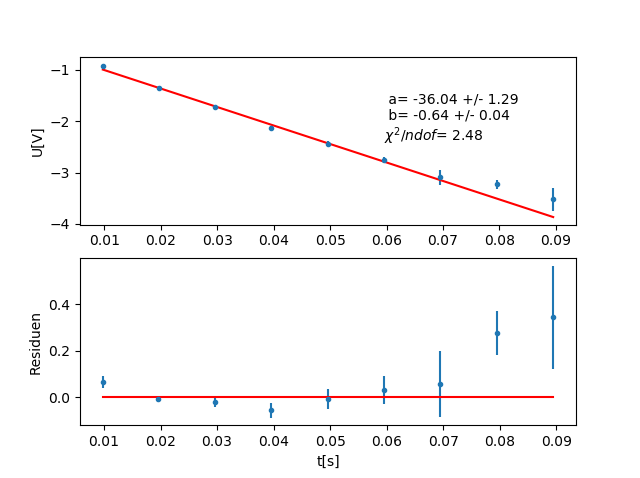
\includegraphics[scale=0.5]{Bilder/T2Anhang/T2log5.png}
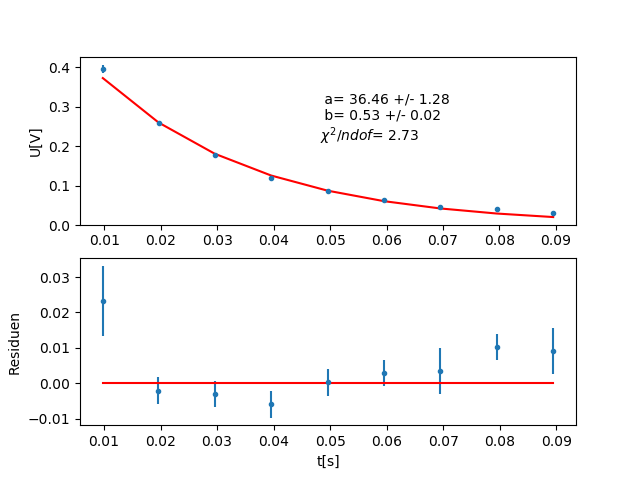
\includegraphics[scale=0.5]{Bilder/T2Anhang/T2exp5.png}
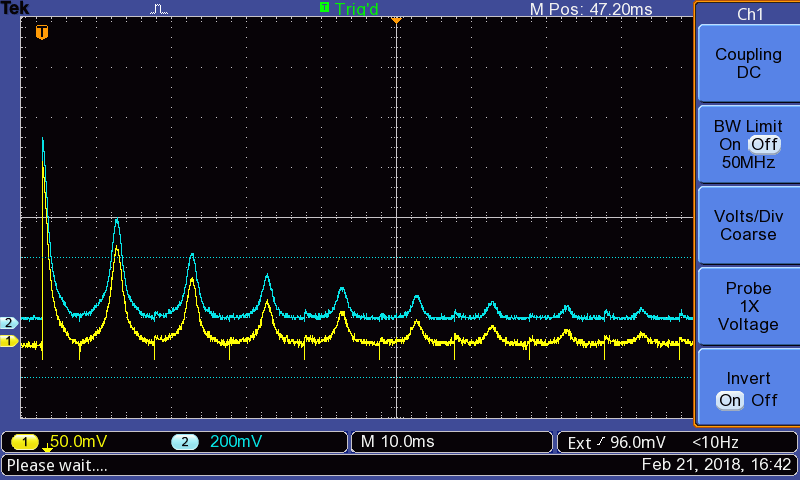
\includegraphics[scale=0.5]{Bilder/T2Anhang/T2plot5.png}
\caption{Daten von der M-G Messung mit $\tau = 5$}
\end{figure}

\begin{figure}
\centering
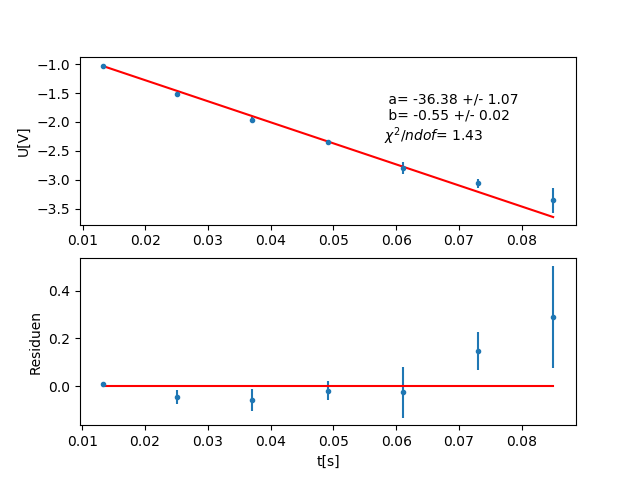
\includegraphics[scale=0.5]{Bilder/T2Anhang/T2log6.png}
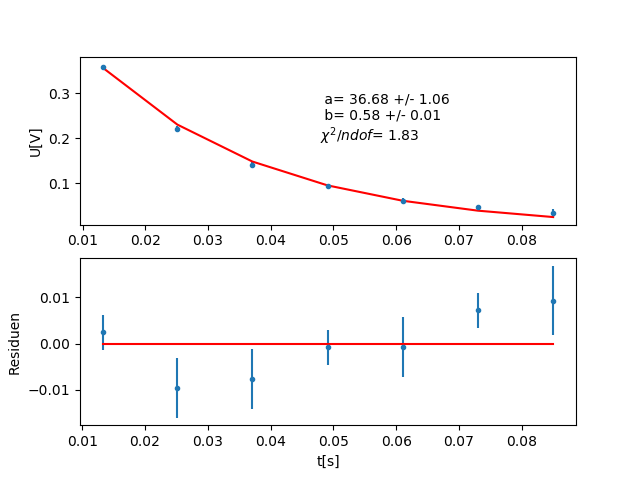
\includegraphics[scale=0.5]{Bilder/T2Anhang/T2exp6.png}
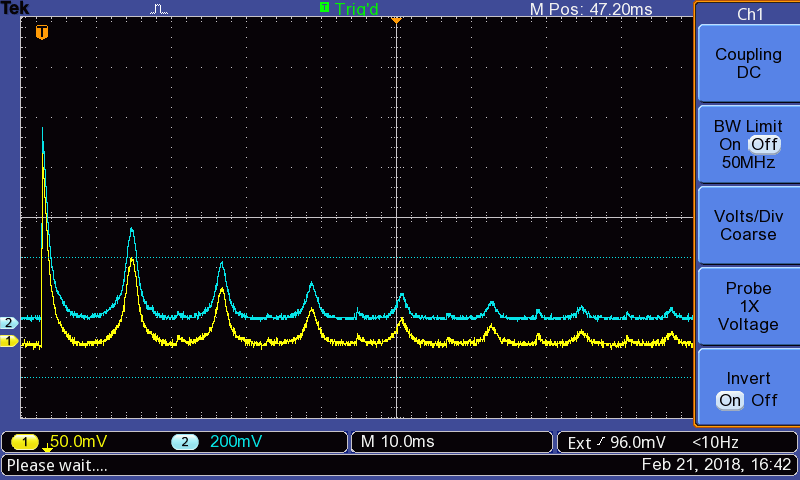
\includegraphics[scale=0.5]{Bilder/T2Anhang/T2plot6.png}
\caption{Daten von M-G für $\tau = 6$}
\end{figure}

\begin{figure}
\centering
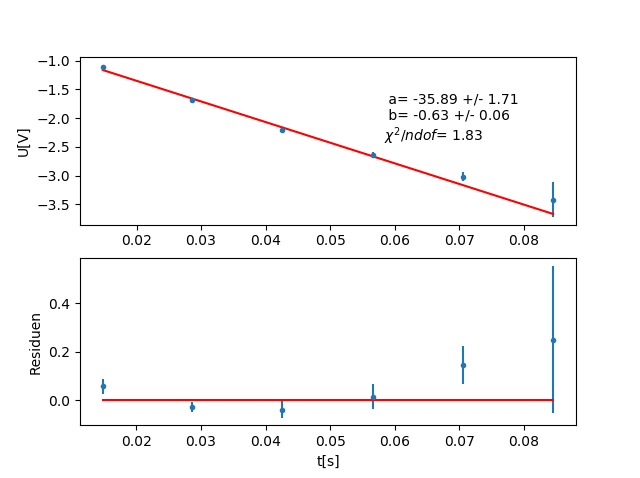
\includegraphics[scale=0.5]{Bilder/T2Anhang/T2log7.png}
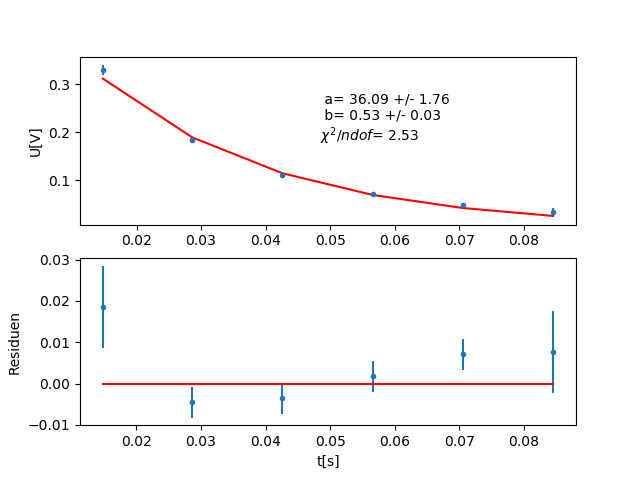
\includegraphics[scale=0.5]{Bilder/T2Anhang/T2exp7.png}
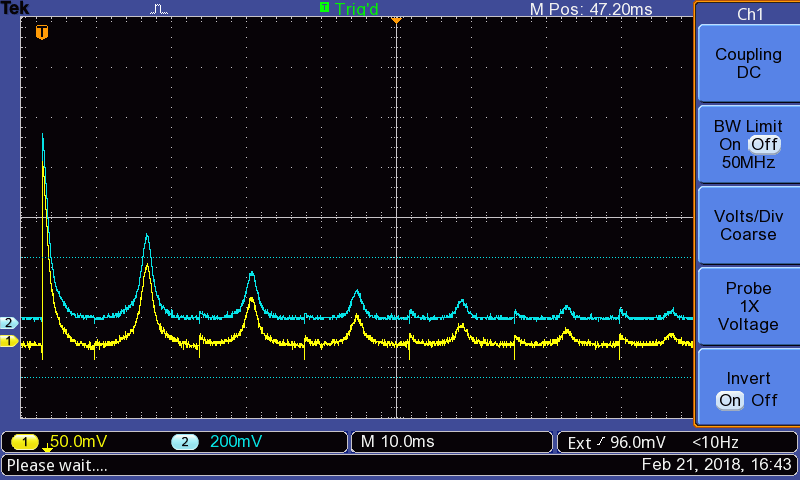
\includegraphics[scale=0.5]{Bilder/T2Anhang/T2plot7.png}
\caption{Daten von M-G für $\tau = 7$}
\end{figure}


\begin{figure}
\centering
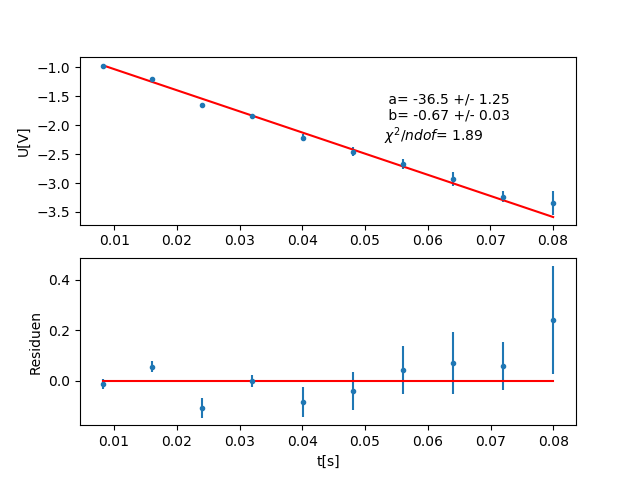
\includegraphics[scale=0.5]{Bilder/T2Anhang/T2log4alt.png}
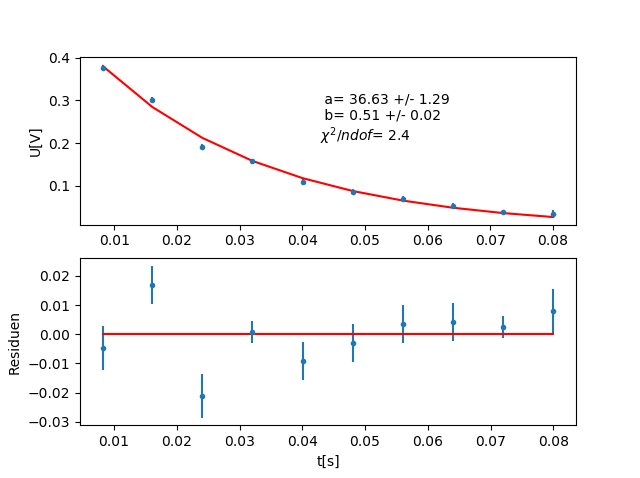
\includegraphics[scale=0.5]{Bilder/T2Anhang/T2exp4alt.png}
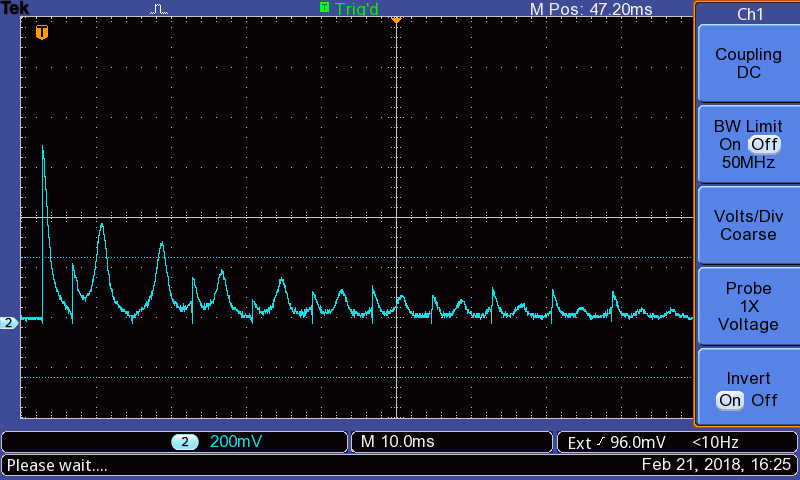
\includegraphics[scale=0.5]{Bilder/T2Anhang/T2plot4alt.png}
\caption{Daten von M-G(alt.) für $\tau = 4$}
\end{figure}


\begin{figure}
\centering
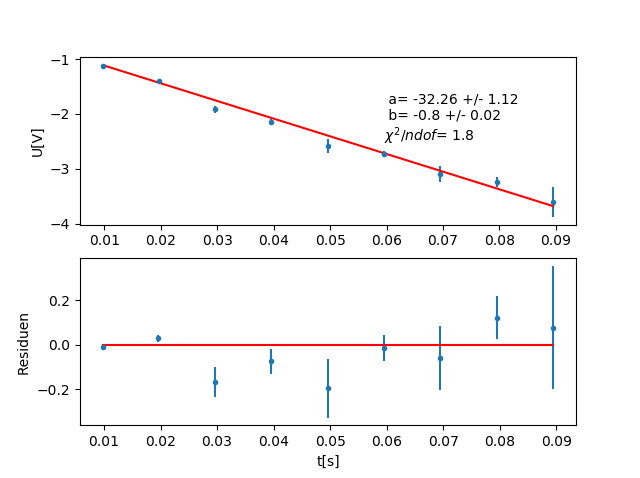
\includegraphics[scale=0.5]{Bilder/T2Anhang/T2log5alt.png}
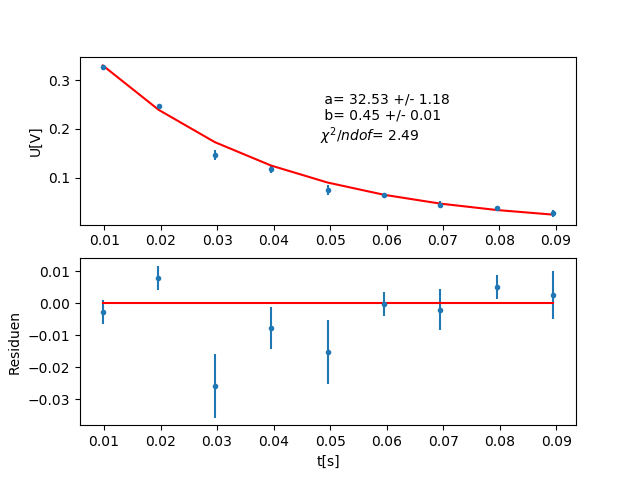
\includegraphics[scale=0.5]{Bilder/T2Anhang/T2exp5alt.png}
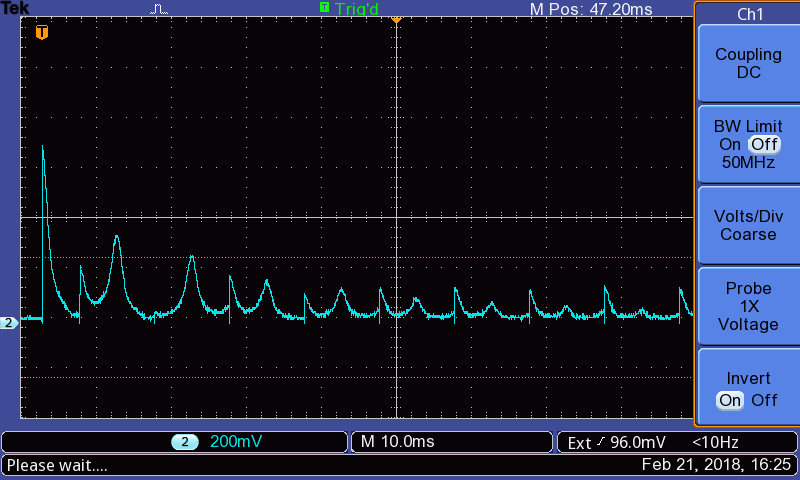
\includegraphics[scale=0.5]{Bilder/T2Anhang/T2plot5alt.png}
\caption{Daten von M-G(alt.) für $\tau = 5$}
\end{figure}


\begin{figure}
\centering
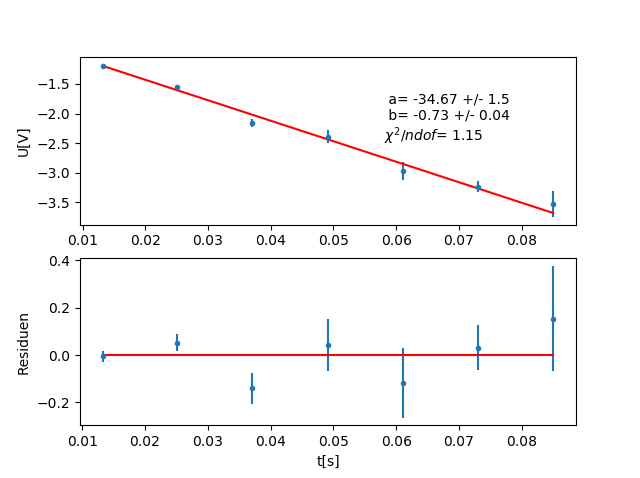
\includegraphics[scale=0.5]{Bilder/T2Anhang/T2log6alt.png}
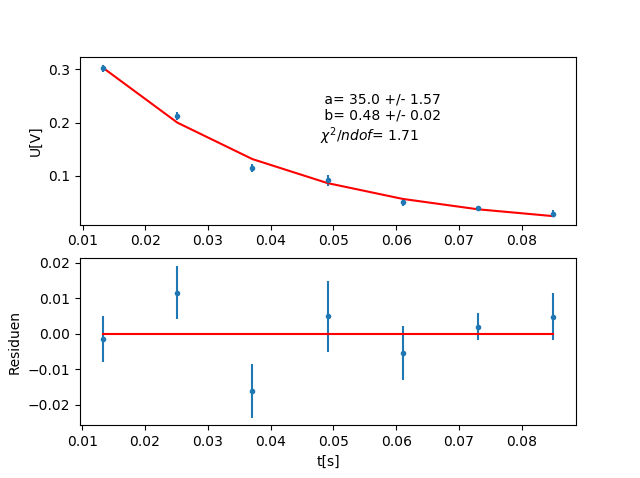
\includegraphics[scale=0.5]{Bilder/T2Anhang/T2exp6alt.png}
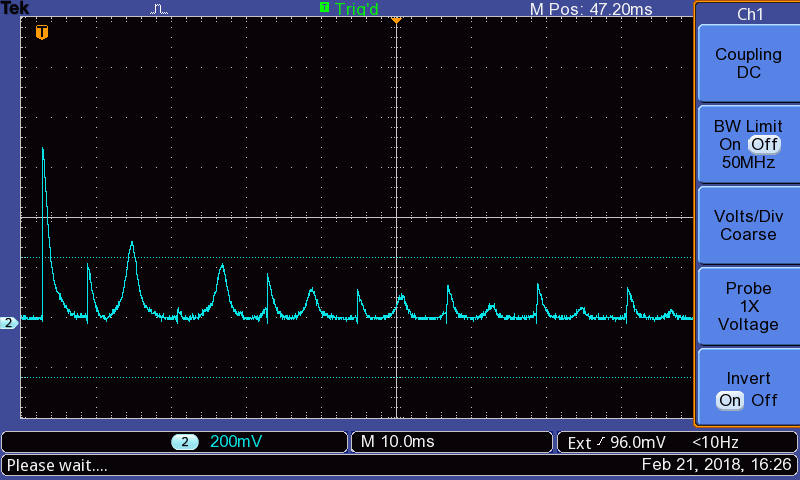
\includegraphics[scale=0.5]{Bilder/T2Anhang/T2plot6alt.png}
\caption{Daten von M-G(alt.) für $\tau = 6$}
\end{figure}


\begin{figure}
\centering
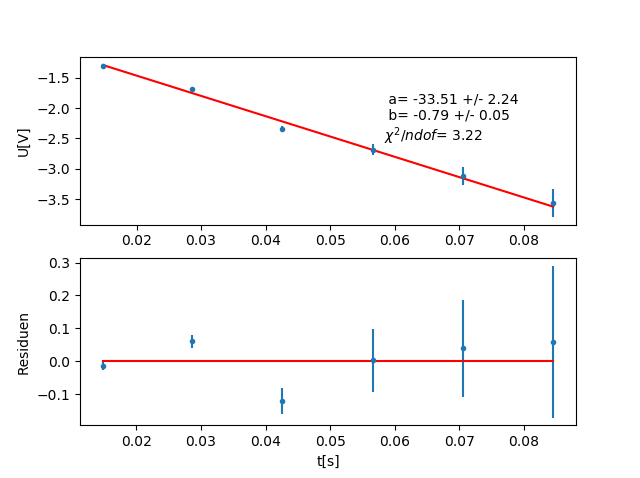
\includegraphics[scale=0.5]{Bilder/T2Anhang/T2log7alt.png}
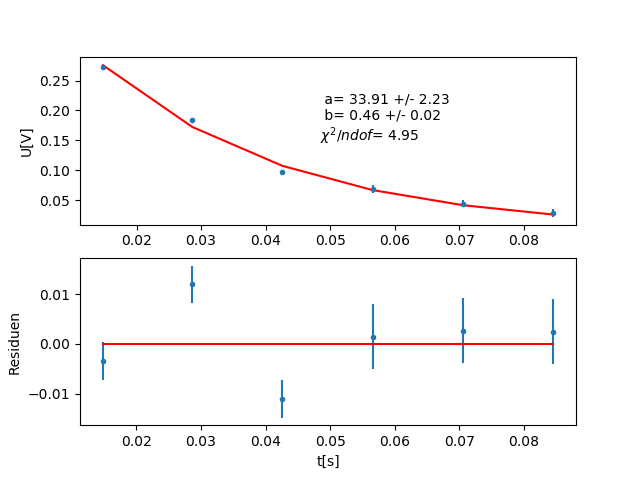
\includegraphics[scale=0.5]{Bilder/T2Anhang/T2exp7alt.png}
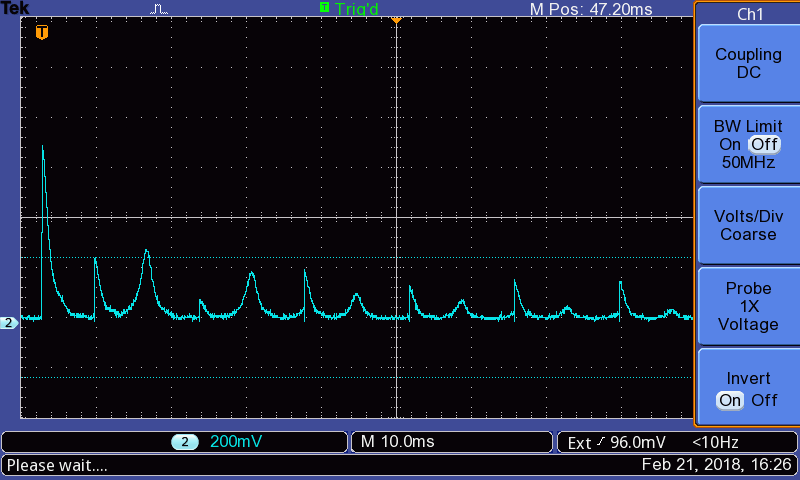
\includegraphics[scale=0.5]{Bilder/T2Anhang/T2plot7alt.png}
\caption{Daten von M-G(alt.) für $\tau = 7$}
\end{figure}

\begin{figure}
\centering
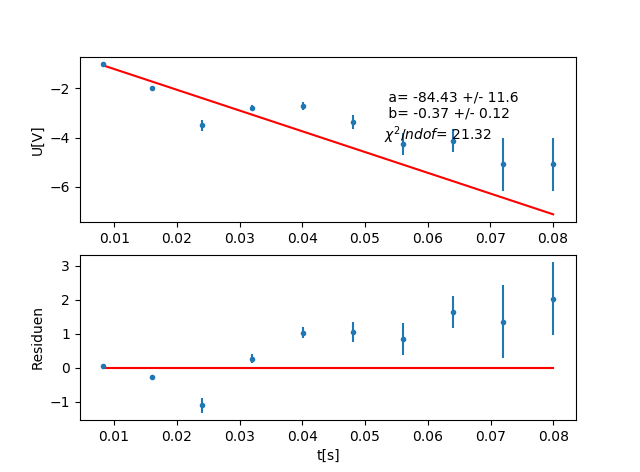
\includegraphics[scale=0.5]{Bilder/T2Anhang/T2CPlin.png}
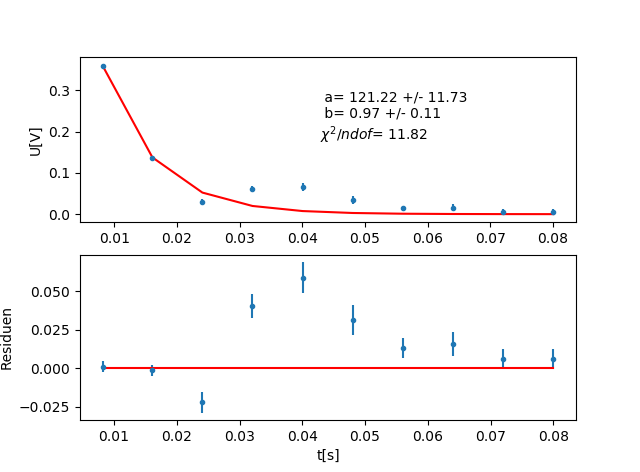
\includegraphics[scale=0.5]{Bilder/T2Anhang/T2CPexp.png}
\includegraphics[scale=0.5]{Bilder/T2Anhang/T2CP.png}
\caption{Daten von C-P(alt.) für $\tau = 4$}
\end{figure}

\begin{figure}
\centering
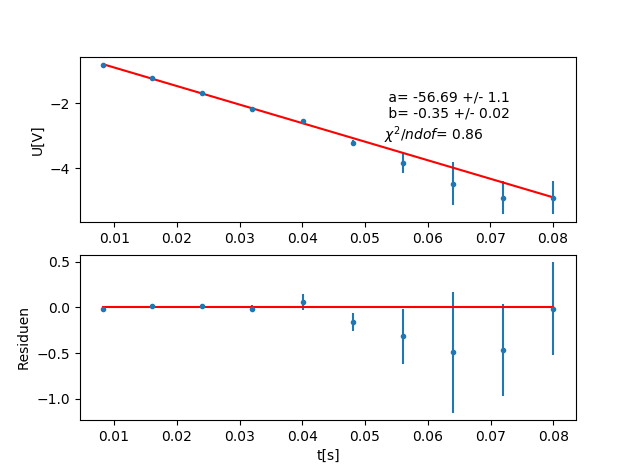
\includegraphics[scale=0.5]{Bilder/T2Anhang/T2CPlinalt.png}
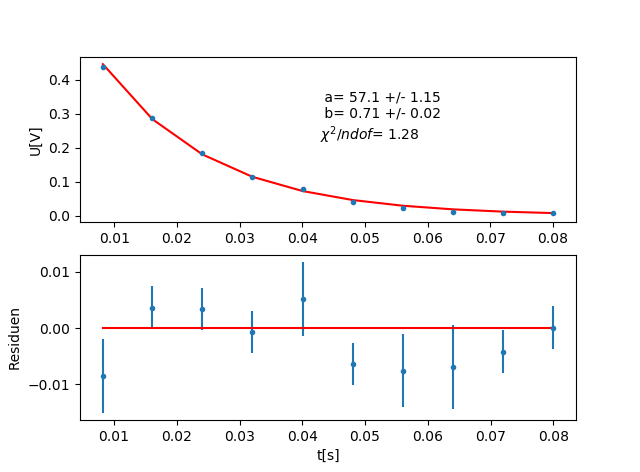
\includegraphics[scale=0.5]{Bilder/T2Anhang/T2CPexpalt.png}
\includegraphics[scale=0.5]{Bilder/T2Anhang/T2CPalt.png}
\caption{Daten von C-P für $\tau = 4$}
\end{figure}

\end{document}